\documentclass[15pt]{beamer}

\usepackage{fancyvrb}

%% Text Handling
\usepackage[utf8]{inputenc}
\usepackage{xspace}
\usepackage{caption}

%% Graphs
\usepackage{tikz}
\usepackage{xcolor}
\usepackage{color}

%% Math
\usepackage{amsmath}
\usepackage{algorithm}

\usetikzlibrary{positioning, arrows, shapes}

\newcommand{\TheTitle}{Merge-Tree}
\newcommand{\TheSubtitle}{Visualizing the Integration of Commits into Linux}
\newcommand{\TheAuthors}{Evan Wilde \and Daniel German}
\newcommand{\TheEmails}{etcwilde@uvic.ca, dmg@uvic.ca}


%% Colors

\definecolor{chartblue}{HTML}{3366CC}
\definecolor{chartred}{HTML}{DC3912}
\definecolor{chartyellow}{HTML}{FF9900}
\definecolor{chartgreen}{HTML}{109618}
\definecolor{chartmagenta}{HTML}{990099}
\definecolor{chartpurple}{HTML}{3B3EAC}

%% Title information
\title{\TheTitle}
\subtitle{\TheSubtitle}
\author[Wilde, German]{\TheAuthors}
\institute{University of Victoria}
\date{}

\setbeamertemplate{footline}[frame number]

\begin{document}
\frame{\titlepage}

\begin{frame}
  \frametitle{Motivation}
  \begin{columns}
    \column{0.5\textwidth}
    \begin{itemize}
      \item 900 Root merges per year
      \item 50K - 70K Commits per year
      \item DAG is very complex
    \end{itemize}
    \column{0.5\textwidth}
    \includegraphics[width=\textwidth]{figures/042dd_DAG.png}
  \end{columns}
\end{frame}

\begin{frame}
  \frametitle{Model}
  \begin{center}
    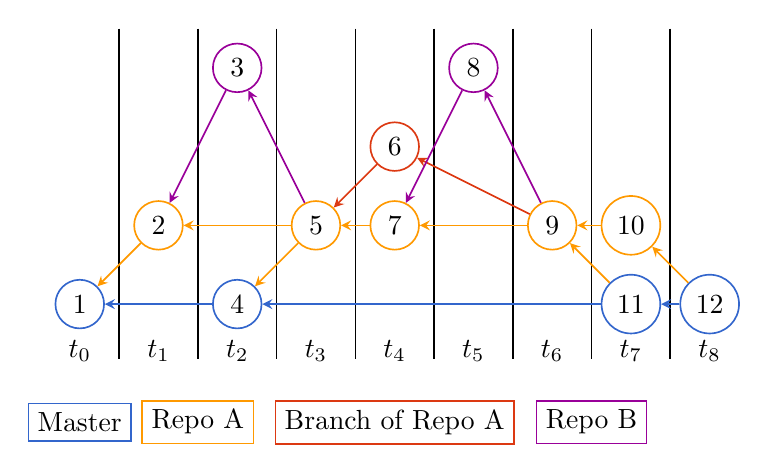
\begin{tikzpicture}[auto, on grid, semithick, state/.style={circle, text=black}]
      \foreach \x in {0, 1, 2, 3, 4, 5, 6, 7}
      \draw[shift={(\x + 0.5, -0.5)}, color=black] (0cm, 4cm) -- (0pt, -0.2cm);

      \node[state, draw=chartblue] (1) {1};
      \node[state, draw=chartyellow, above right= of 1] (2) {2};
      \node[state, draw=chartmagenta, above right= 2cm and 1cm of 2] (3) {3};
      \node[state, draw=chartblue, right= 2cm of 1] (4) {4};
      \node[state, draw=chartyellow, above right=of 4] (5) {5};
      \node[state, draw=chartred, above right=of 5] (6) {6};
      \node[state, draw=chartyellow, right=of 5] (7) {7};
      \node[state, draw=chartmagenta, above right= 2cm and 1cm of 7](8) {8};
      \node[state, draw=chartyellow, right= 2cm of 7] (9) {9};
      \node[state, draw=chartyellow, right=of 9] (10) {10};
      \node[state, draw=chartblue, below right=of 9] (11) {11};
      \node[state, draw=chartblue, below right=of 10] (12) {12};

      \draw (12) edge[chartblue, -stealth] (11) edge[chartyellow, -stealth] (10);
      \draw (11) edge[chartblue, -stealth] (4) edge[chartyellow, -stealth] (9);
      \draw (10) edge[chartyellow, -stealth] (9);
      \draw (9) edge[chartmagenta, -stealth] (8) edge[chartred, -stealth] (6)
      edge[chartyellow, -stealth] (7);
      \draw (8) edge[chartmagenta, -stealth] (7);
      \draw (7) edge[chartyellow, -stealth] (5);
      \draw (6) edge[chartred, -stealth] (5);
      \draw (5) edge[chartmagenta, -stealth] (3) edge[chartyellow,-stealth] (2)
      edge[chartyellow, -stealth] (4);
      \draw (4) edge[chartblue, -stealth] (1);
      \draw (3) edge[chartmagenta, -stealth] (2);
      \draw (2) edge[chartyellow, -stealth] (1);

      \node [draw=chartblue, below = 1.5cm of 1] (l1) {Master};
      \node [draw=chartyellow, right = 1.5cm of l1] (l2) {Repo A};
      \node [draw=chartred, right = 2.5cm of l2] (l3) {Branch of Repo A};
      \node [draw=chartmagenta, right= 2.5cm of l3] (l4) {Repo B};

      \foreach \x in {0, 1, 2, 3, 4, 5, 6, 7, 8}
      \node[shift={(\x, -0.6)}, color=black] {$t_\x$};
    \end{tikzpicture}
  \end{center}
\end{frame}

\begin{frame}
  \frametitle{Model}
  \begin{center}
    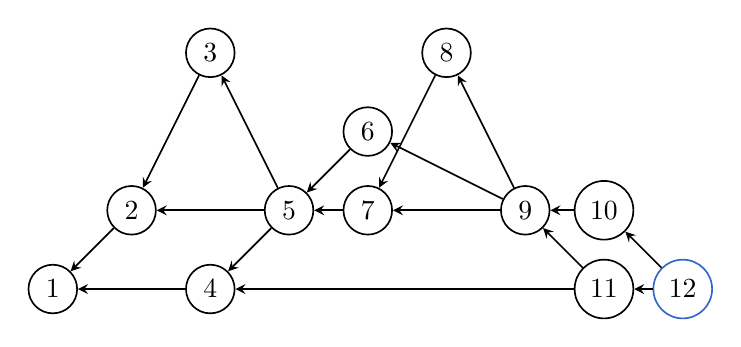
\begin{tikzpicture}[auto, on grid, semithick, state/.style={circle, text=black, draw=black}]
      \node[state] (1) {1};
      \node[state, above right= of 1] (2) {2};
      \node[state, above right= 2cm and 1cm of 2] (3) {3};
      \node[state, right= 2cm of 1] (4) {4};
      \node[state, above right=of 4] (5) {5};
      \node[state, above right=of 5] (6) {6};
      \node[state, right=of 5] (7) {7};
      \node[state, above right= 2cm and 1cm of 7](8) {8};
      \node[state, right= 2cm of 7] (9) {9};
      \node[state, right=of 9] (10) {10};
      \node[state, below right=of 9] (11) {11};
      \node[state, draw=chartblue, below right=of 10] (12) {12};

      \draw (12) edge[-stealth] (11) edge[-stealth] (10);
      \draw (11) edge[-stealth] (4) edge[-stealth] (9);
      \draw (10) edge[-stealth] (9);
      \draw (9) edge[-stealth] (8) edge[-stealth] (6)
      edge[-stealth] (7);
      \draw (8) edge[-stealth] (7);
      \draw (7) edge[-stealth] (5);
      \draw (6) edge[-stealth] (5);
      \draw (5) edge[-stealth] (3) edge[-stealth] (2)
      edge[-stealth] (4);
      \draw (4) edge[-stealth] (1);
      \draw (3) edge[-stealth] (2);
      \draw (2) edge[-stealth] (1);
    \end{tikzpicture}
  \end{center}
\end{frame}

\begin{frame}
  \frametitle{Model}
  \begin{center}
    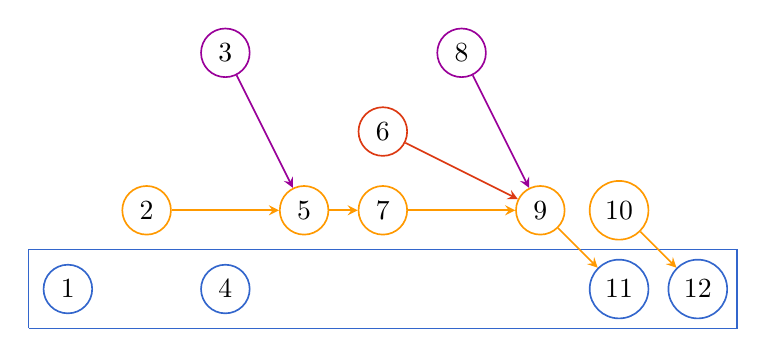
\begin{tikzpicture}[auto, on grid, semithick, state/.style={circle, text=black}]

      \draw[chartblue]
      (-0.5, -0.5) -- (8.5, -0.5) -- (8.5, 0.5) -- (-0.5, 0.5) -- (-0.5, -0.5);

      \node[state, draw=chartblue] (1) {1};
      \node[state, draw=chartyellow, above right= of 1] (2) {2};
      \node[state, draw=chartmagenta, above right= 2cm and 1cm of 2] (3) {3};
      \node[state, draw=chartblue, right= 2cm of 1] (4) {4};
      \node[state, draw=chartyellow, above right=of 4] (5) {5};
      \node[state, draw=chartred, above right=of 5] (6) {6};
      \node[state, draw=chartyellow, right=of 5] (7) {7};
      \node[state, draw=chartmagenta, above right= 2cm and 1cm of 7](8) {8};
      \node[state, draw=chartyellow, right= 2cm of 7] (9) {9};
      \node[state, draw=chartyellow, right=of 9] (10) {10};
      \node[state, draw=chartblue, below right=of 9] (11) {11};
      \node[state, draw=chartblue, below right=of 10] (12) {12};

      \draw (2) edge[chartyellow, -stealth] (5)
      (3) edge[chartmagenta, -stealth](5)
      (5) edge[chartyellow, -stealth] (7)
      (7) edge[chartyellow, -stealth] (9)
      (6) edge[chartred, -stealth] (9)
      (8) edge[chartmagenta, -stealth] (9)
      (9) edge[chartyellow, -stealth] (11)
      (10) edge[chartyellow, -stealth] (12);
    \end{tikzpicture}
  \end{center}
\end{frame}

\begin{frame}
  \frametitle{Heuristic}

  \begin{enumerate}
    \item Identify the master branch
    \item For every commit, recursively calculate shortest path to master
  \end{enumerate}
\end{frame}

\begin{frame}
  \frametitle{Heuristic}
  \begin{center}
    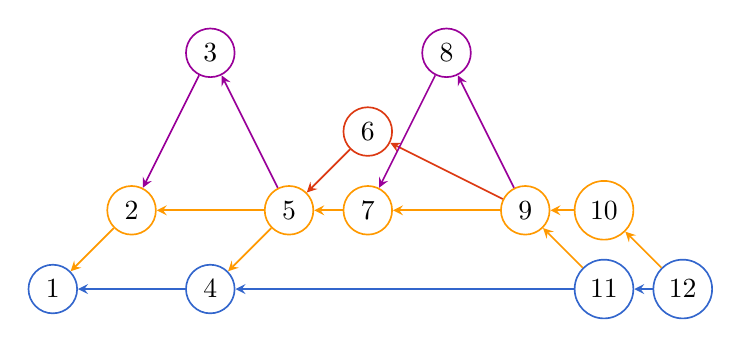
\begin{tikzpicture}[auto, on grid, semithick, state/.style={circle, text=black}]
      \node[state, draw=chartblue] (1) {1};
      \node[state, draw=chartyellow, above right= of 1] (2) {2};
      \node[state, draw=chartmagenta, above right= 2cm and 1cm of 2] (3) {3};
      \node[state, draw=chartblue, right= 2cm of 1] (4) {4};
      \node[state, draw=chartyellow, above right=of 4] (5) {5};
      \node[state, draw=chartred, above right=of 5] (6) {6};
      \node[state, draw=chartyellow, right=of 5] (7) {7};
      \node[state, draw=chartmagenta, above right= 2cm and 1cm of 7](8) {8};
      \node[state, draw=chartyellow, right= 2cm of 7] (9) {9};
      \node[state, draw=chartyellow, right=of 9] (10) {10};
      \node[state, draw=chartblue, below right=of 9] (11) {11};
      \node[state, draw=chartblue, below right=of 10] (12) {12};

      \draw (12) edge[chartblue, -stealth] (11) edge[chartyellow, -stealth] (10);
      \draw (11) edge[chartblue, -stealth] (4) edge[chartyellow, -stealth] (9);
      \draw (10) edge[chartyellow, -stealth] (9);
      \draw (9) edge[chartmagenta, -stealth] (8) edge[chartred, -stealth] (6)
      edge[chartyellow, -stealth] (7);
      \draw (8) edge[chartmagenta, -stealth] (7);
      \draw (7) edge[chartyellow, -stealth] (5);
      \draw (6) edge[chartred, -stealth] (5);
      \draw (5) edge[chartmagenta, -stealth] (3) edge[chartyellow,-stealth] (2)
      edge[chartyellow, -stealth] (4);
      \draw (4) edge[chartblue, -stealth] (1);
      \draw (3) edge[chartmagenta, -stealth] (2);
      \draw (2) edge[chartyellow, -stealth] (1);
    \end{tikzpicture}
  \end{center}
\end{frame}

\begin{frame}[t]
  \frametitle{Heuristic Verification}
  \includegraphics[width=\textwidth]{verbatim.pdf}
\end{frame}

\begin{frame}
  \frametitle{Heuristic Results}
  \begin{itemize}
    \item Five merges had inaccurate logs causing problems
    \item Heursitic identified 79 merges to non-master branches
    \item Worked perfectly until 2007
    \item Foxtrot breaks heuristic in 2006
  \end{itemize}
\end{frame}

\begin{frame}
  \frametitle{Heuristic Results}
  \begin{itemize}
    \item Correctly identified 16860 commits
    \item Failed in 1542 commits before Dec. 12 2006
    \item 836 appear to be correct
  \end{itemize}
\end{frame}

\begin{frame}
  \frametitle{Tool}
  \begin{itemize}
    \item Top-to-bottom
      \begin{itemize}
        \item Aggregate
      \end{itemize}
    \item Bottom-to-top
      \begin{itemize}
        \item See flow into master
      \end{itemize}
  \end{itemize}
\end{frame}

\begin{frame}
  \frametitle{An Example}
  \begin{center}
    \includegraphics[width=0.9\textwidth]{figures/042dd_DAG.png}
  \end{center}
\end{frame}

\begin{frame}
  \frametitle{An Example}
  \begin{center}
    \includegraphics[width=\textwidth]{figures/042d/042dd_DAG_focus.png}
  \end{center}
\end{frame}

\begin{frame}
  \frametitle{042dd List Tree}
  \begin{center}
    \includegraphics[width=\textwidth]{figures/042d/list_tree.png}
  \end{center}
\end{frame}

\begin{frame}
  \frametitle{042dd Reingold Tilford Tree}
  \begin{center}
    \includegraphics[width=0.9\textwidth]{figures/042d/reingold_tree.pdf}
  \end{center}
\end{frame}

\begin{frame}
  \frametitle{042dd Bubble Tree}
  \begin{center}
    \includegraphics[width=0.7\textwidth]{figures/042d/bubble_tree.pdf}
  \end{center}
\end{frame}

\begin{frame}
  \frametitle{042dd Summary}
  \begin{center}
    \includegraphics[width=\textwidth]{figures/042d/summary.png}
  \end{center}
\end{frame}

\begin{frame}
  \frametitle{042dd Files}
  \begin{center}
    \includegraphics[width=\textwidth]{figures/042d/files.png}
  \end{center}
\end{frame}

\begin{frame}
  \frametitle{042dd Modules}
  \begin{center}
    \includegraphics[width=\textwidth]{figures/042d/modules.png}
  \end{center}
\end{frame}

\begin{frame}
  \frametitle{042dd Authors}
  \begin{center}
    \includegraphics[width=\textwidth]{figures/042d/042dd_authors.png}
  \end{center}
\end{frame}

\begin{frame}
  \frametitle{Challenges}
  \begin{itemize}
    \item Tree Labels
    \item CID's are long and unrecognizable
    \item Differences in relative scale
  \end{itemize}
\end{frame}

\begin{frame}
  \frametitle{Challenges}
  \begin{center}
    \includegraphics[width=0.7\textwidth]{figures/4dc4_tree.pdf}
  \end{center}
\end{frame}

\begin{frame}
  \frametitle{Conclusion}
  Merge trees are a much simpler way to inspect how a commit flows into the master
  branch.

\end{frame}


\end{document}
